\documentclass[11pt,a4paper]{article}
\usepackage[margin=2cm]{geometry}
\usepackage[T1]{fontenc}
\usepackage{lmodern}
\usepackage{microtype}
\usepackage{graphicx}
\usepackage{booktabs}
\usepackage{tabularx}
\usepackage{xcolor}
\usepackage{caption}
\usepackage{float}
\usepackage{enumitem}
\usepackage[hidelinks]{hyperref}

\definecolor{stock}{HTML}{C0392B}
\definecolor{patched}{HTML}{1F5FA8}
\captionsetup{font=small,labelfont=bf}
\setlist{itemsep=1pt,topsep=3pt}
\newcommand{\maxfs}{\ensuremath{\mathit{maxFS}}}
\newcommand{\cwnd}{\ensuremath{\mathit{cwnd}}}
\newcommand{\ssthresh}{\ensuremath{\mathit{ssthresh}}}
\newcommand{\smss}{\ensuremath{\mathit{SMSS}}}

\title{\textbf{Rate-Limited Sender Increase in MsQuic CUBIC}\\[2pt]
  \large Project summary}
\author{Abhiram Suresh}
\date{November 2026}
\setlength{\textfloatsep}{8pt plus 2pt}

\begin{document}
\maketitle
\vspace{-1em}

\begin{abstract}
\noindent
We implemented the rules of \texttt{draft-ietf-ccwg-ratelimited-increase-11}
in the CUBIC congestion controller of Microsoft's MsQuic. When an application
sends less than its congestion window allows, stock MsQuic keeps growing the
window anyway, then releases it all at once when the application becomes
busy again. Our patch (34 lines of C) bounds the window by what the sender has
actually used. The network evaluation also uncovered an \emph{unrelated bug}
in upstream MsQuic: an unsigned underflow in CUBIC's Reno-friendly
accumulator that makes the window grow by one packet per ACK. We fixed it
too. In 420 emulated runs, after 28\,s of rate-limited sending the window at
resumption drops from 670 to 166\,KB and the data lost from 1094 to 32\,KB.
The one cost: on a 50\,Mbit/s path with a shallow queue, an 8\,MB transfer
takes 23\,\% longer.
\end{abstract}

\section{Problem}

Many applications are \emph{rate-limited}: video players, RPC clients,
games and heartbeats send less than the congestion window (\cwnd) would allow.
CUBIC grows \cwnd\ as a function of time since the last loss, on every ACK,
so the window keeps growing even though the network never carried that much
of the sender's data. Figure~\ref{fig:hook} shows this on our testbed. During 28\,s at
about 25\,KB in flight, stock MsQuic's window grows from 150 to 670\,KB. When
the application then has 8\,MB to send, it releases that whole window in one
round trip, overflows the bottleneck queue, and loses over 1\,MB of data.

\begin{figure}[t]
  \centering
  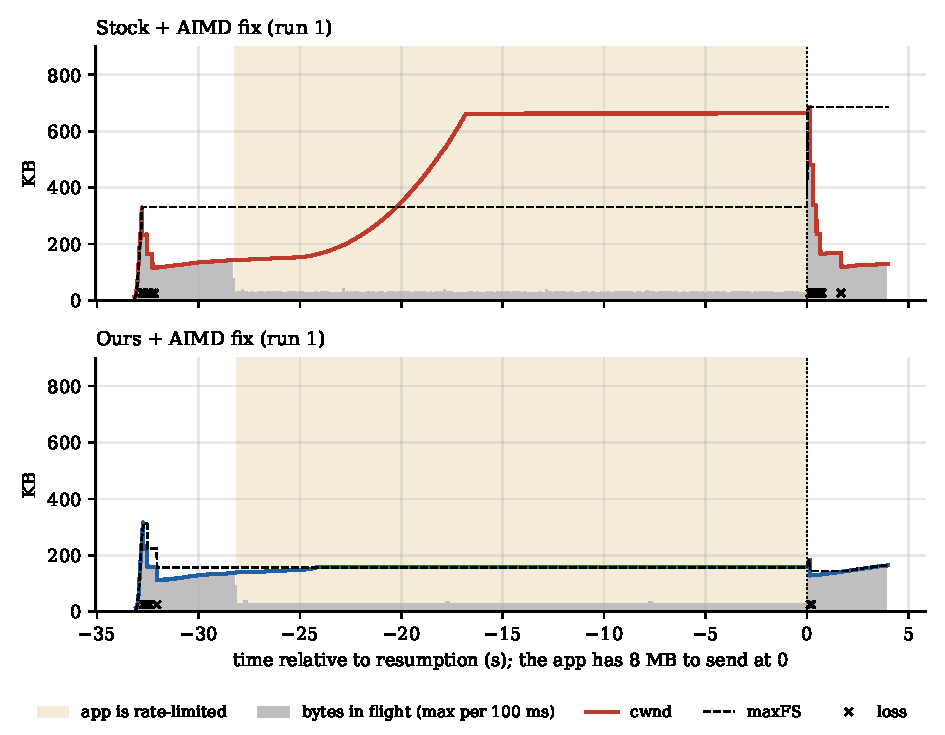
\includegraphics[width=0.55\textwidth]{figures/clean_timeline.pdf}
  \caption{One run of each build (both with the accumulator fix of
    Section~\ref{sec:bug}). Shaded: rate-limited phase; the application
    resumes bulk sending at $t = 0$.}
  \label{fig:hook}
\end{figure}

\section{What the draft requires and what MsQuic did}

The draft defines \maxfs, the largest flight size since the last window
reduction, and requires: \maxfs\ is reset to 0 whenever \cwnd\ is reduced;
in slow start $\cwnd \le 2\cdot\maxfs$; in congestion avoidance
$\cwnd \le \maxfs + 1\,\smss$. MsQuic already tracked \maxfs\
(\texttt{BytesInFlightMax}) and capped \cwnd\ at $2\cdot\maxfs$, but with two
gaps:
\begin{itemize}
  \item \textbf{Gap 1:} \maxfs\ was never reset, so after a loss the cap was
        based on the flight that had just caused the loss.
  \item \textbf{Gap 2:} the cap was $2\cdot\maxfs$ in congestion avoidance too,
        twice what the draft allows.
\end{itemize}

\section{Our changes}

\begin{table}[H]
\centering\small
\begin{tabularx}{\textwidth}{@{}l l X@{}}
\toprule
 & Where in \texttt{cubic.c} & Change \\
\midrule
C1 & \texttt{OnCongestionEvent} & Save \maxfs\ (for undo), then reset it to 0. Covers loss, ECN and persistent congestion. \\
C2 & \texttt{OnDataLost}, \texttt{OnEcn} & Re-measure \maxfs\ from the flight that is still in the network after the reduction. \\
C3 & \texttt{OnDataAcknowledged} & Cap \cwnd\ at $2\cdot\maxfs$ in slow start and $\maxfs + \smss$ in congestion avoidance. \\
C4 & \texttt{OnDataAcknowledged} & Never let the cap go below QUIC's 2-packet minimum window (RFC 9002). \\
C5 & \texttt{OnSpuriousCongestionEvent} & Restore \maxfs\ when a loss turns out to be spurious. \\
\bottomrule
\end{tabularx}
\caption{The five changes (34 lines of code). \ssthresh\ is deliberately left
  unchanged when the cap binds: lowering it, which we tried first, slowed later
  ramp-up (9 instead of 23 packets sent in the 15th round trip).}
\label{tab:changes}
\end{table}

\section{Per-change evaluation}

We drove MsQuic's own CUBIC code through
deterministic scenarios in its unit-test harness, against stock, the full
patch, and the patch with one change disabled. In the main scenario (loss at
40 packets, then 4 packets per round trip for 10\,s; Figure~\ref{fig:scenA})
stock CUBIC grows \cwnd\ to 76 packets and releases a 76-packet burst; the
patch holds it at 29. Removing C1--C2 gives 41, removing the CA cap gives 56.
Each of the other changes has its own scenario where removing it breaks
something: without C4 a heartbeat sender's window drops to 600\,B (less than
one packet), and without C5 an undone spurious loss still cuts \cwnd\ from
29.5 to 22 packets.

\begin{figure}[H]
  \centering
  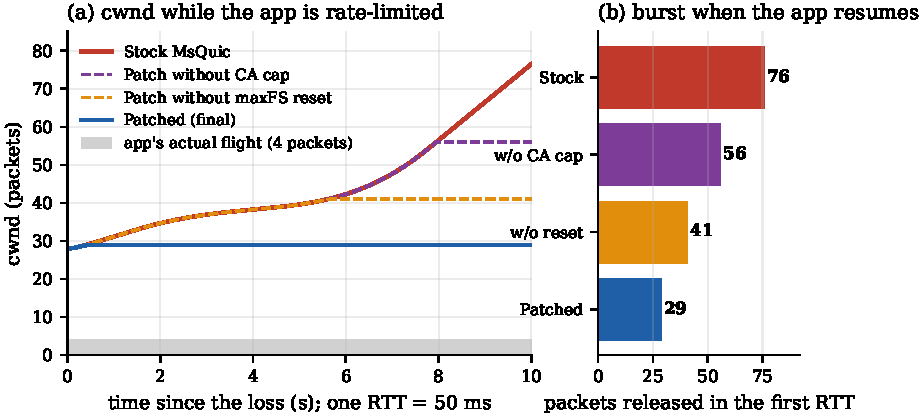
\includegraphics[width=0.66\textwidth]{figures/scenario_a.pdf}
  \caption{Scenario A. (a) \cwnd\ while only 4 packets per round are in flight;
    (b) burst when the application resumes. Both fixes are needed.}
  \label{fig:scenA}
\end{figure}

\section{An upstream bug found along the way}
\label{sec:bug}

The first network campaign gave a result our patch could not explain: with a
competing TCP flow, our sender sometimes grew its window faster than stock.
The cause is in MsQuic's Reno-friendly (AIMD) window:
\begin{center}\small
\texttt{AimdWindow += SMSS; AimdAccumulator -= AimdWindow;}
\end{center}
The code subtracts the window \emph{after} growing it. Both fields are
\texttt{uint32}, so when an ACK makes the accumulator exceed the window by less
than one packet, the subtraction wraps to about $4.3\cdot10^{9}$. From then on
the AIMD window grows by one packet on \emph{every} ACK, which is exponential
growth in congestion avoidance. In stock runs 11--33\,\% of all window
increases in congestion avoidance were a full packet on a single ACK; with the
fix, under 6\,\%. The bug is still present in upstream \texttt{main}; the upstream unit
test sizes its ACKs so that the wrap never happens. We swapped the two lines and
added a unit test that fails on the old code (MsQuic commit
\texttt{1ca13e9d7}, \texttt{patches/0004}).

\section{Network evaluation}

\paragraph{Testbed.} Linux namespaces form a dumbbell with a netem bottleneck
(10--50\,Mbit/s, 11--81\,ms RTT, 100-packet drop-tail queue, segmentation
offloads off). The QUIC sender sends 3\,MB, then 6000\,B every 10\,ms, then
8\,MB. A ping flow, and in one setting an \texttt{iperf3} TCP CUBIC flow,
share the bottleneck. We ran 10 runs per setting with rotating build order: a
sweep over 11 settings (stock vs.\ patched, 220 runs), and a four-build
experiment (5 settings $\times$ 4 builds, 200 runs) that separates the effect of
our patch from that of the bug fix.

\paragraph{Sweep.} We measure how long the sender was \emph{really}
rate-limited, from its last cwnd-limited send to resumption (the 3\,MB start-up
takes about 5\,s to drain). With under 1\,s both builds behave the same: CUBIC
has not had time to grow the window. From 6\,s on,
at every RTT and rate, stock resumes with 590--760\,KB, against
145--260\,KB for the patch, and loses 1.1--3.8\,MB instead of 31--145\,KB.
Because the queue is short, the harm shows up as loss rather than delay: the
competing ping's maximum RTT differs by only a few milliseconds.

\begin{table}[tbp]
\centering\small
\setlength{\tabcolsep}{5pt}
\begin{tabular}{@{}llccccc@{}}
\toprule
Setting & Metric (median) & Stock & Stock+fix & Patch & Patch+fix & $p$ \\
\midrule
6 s rate-limited & \cwnd\ at resumption (KB) & 668 & 229 & 166 & 166 & $<$0.001 \\
 & data lost after resuming (KB) & 3413 & 82 & 109 & 30 & $<$0.001 \\
28 s rate-limited & \cwnd\ at resumption (KB) & 670 & 671 & 166 & 166 & $<$0.001 \\
 & data lost after resuming (KB) & 1094 & 1094 & 31 & 32 & $<$0.001 \\
RTT 80\,ms & data lost after resuming (KB) & 2800 & 84 & 121 & 40 & $<$0.001 \\
50\,Mbit/s & data lost after resuming (KB) & 3002 & 140 & 105 & 92 & $<$0.001 \\
 & 8\,MB transfer time (s) & 2.07 & 2.04 & 2.17 & 2.50 & $<$0.001 \\
+ TCP flow & QUIC data lost (KB) & 106 & 47 & 123 & 21 & 0.06 \\
 & TCP worst 0.5\,s (Mbit/s) & 6.3 & 13.6 & 6.3 & 14.7 & -- \\
\bottomrule
\end{tabular}
\caption{Four-build experiment, 10 runs per cell. ``+fix'' = with the
  accumulator fix. $p$: permutation test, Patch+fix vs.\ Stock+fix.}
\label{tab:four}
\end{table}

\paragraph{What the four builds show.}
\begin{itemize}
  \item \textbf{After short rate-limited periods, the bug is most of the
        problem.} At 6\,s the fix alone brings stock from 668 to 229\,KB.
        Our patch takes it further to 166\,KB and cuts the loss from 82 to
        30\,KB.
  \item \textbf{After long periods, the draft's rule is what matters.} At
        28\,s the bug fix changes nothing (670\,KB). CUBIC's cubic curve
        alone reaches the stale cap. Only our patch holds the window at the
        166\,KB actually used, cutting loss from 1094 to 32\,KB.
  \item \textbf{With a competing TCP flow, both changes are needed.} Our
        patch without the fix still lets the wrapped accumulator push the
        window up (TCP's worst 0.5\,s: 6.3\,Mbit/s). With both, TCP keeps
        14.7\,Mbit/s and QUIC loses 21 instead of 47\,KB ($p = 0.06$).
  \item \textbf{A cost on high-BDP paths with a shallow queue.} At
        50\,Mbit/s even the patched resume burst overflows the 100-packet
        queue. Starting from a smaller window, the sender ends up with a
        smaller window after the loss, and the 8\,MB transfer takes 2.50
        instead of 2.04\,s. This is the conservative side of the draft.
\end{itemize}

\section{More examples}

Figure~\ref{fig:examples} collects four further examples, each from measured
data.
\begin{itemize}
  \item \textbf{(a) The upstream bug on its own.} In MsQuic's unit-test
        harness, after a loss with the window fully used, stock CUBIC's window
        grows from 67 to 2839\,KB in six round trips: it doubles every round
        trip although it is in congestion avoidance. With the fix it grows
        from 67 to 75\,KB, about one packet per round trip, as CUBIC should.
  \item \textbf{(b) When the problem matters.} Data lost after resuming
        against the time the sender was really rate-limited (sweep campaign,
        before the bug fix, median and IQR of 10 runs). Below 1\,s both builds
        lose almost nothing; from 6\,s on stock loses 1.1--3.8\,MB and the
        patch 31--111\,KB, 26--58 times less.
  \item \textbf{(c) Fairness to TCP.} The worst 0.5\,s of a competing TCP
        flow after our sender resumes, in each of 10 runs. Stock and the patch
        without the bug fix both push TCP down to a median of 6.3\,Mbit/s,
        sometimes to 0; with both fixes TCP keeps 14.7\,Mbit/s, at least its fair share of the 25\,Mbit/s link.
  \item \textbf{(d) ECN instead of loss.} The draft's reset applies to every
        window reduction, including an ECN mark. After the mark, stock grows the
        window from 42 to 57 packets while only 20--24 packets are in flight. The patch
        keeps it between the congestion-avoidance cap ($\maxfs + 1$ packet) and
        \ssthresh: whenever the cap drops \cwnd\ below \ssthresh, CUBIC is back
        in slow start, which the draft caps only at $2\cdot\maxfs$. Lowering
        \ssthresh\ would remove this oscillation but slowed later ramp-up
        (Table~\ref{tab:changes}), so we left it.
\end{itemize}

\begin{figure}[H]
  \centering
  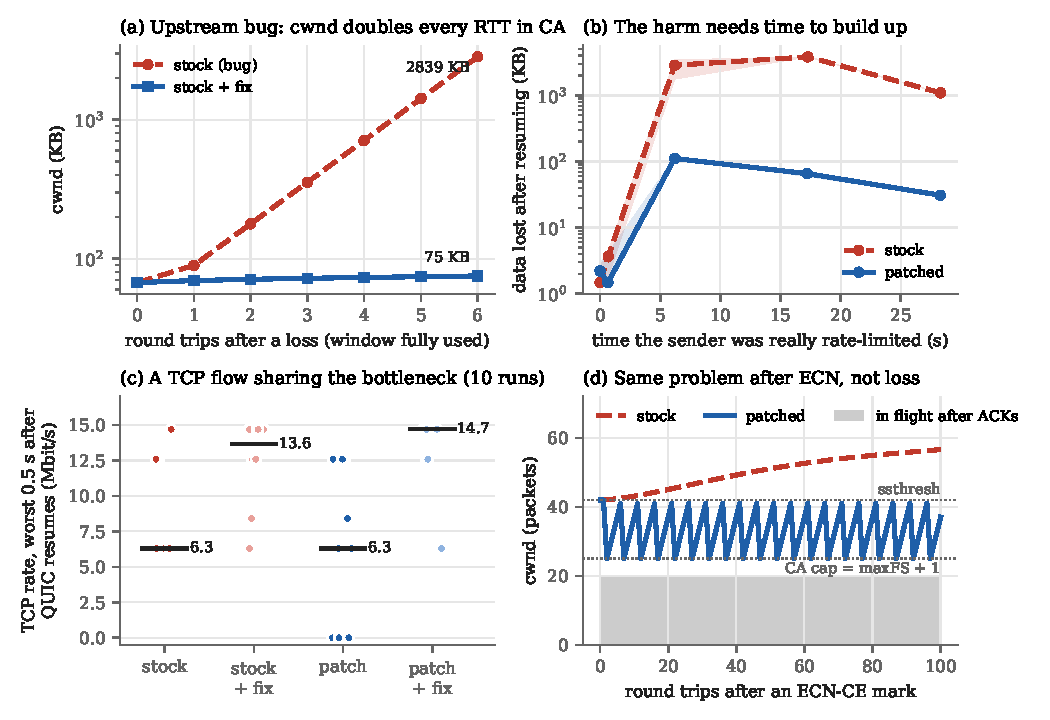
\includegraphics[width=0.95\textwidth]{figures/examples.pdf}
  \caption{Four further examples. (a, d): MsQuic's CUBIC code driven by
    the unit-test harness. (b, c): emulated-network campaigns, 10 runs per
    point; (c) black bars are medians.}
  \label{fig:examples}
\end{figure}

\paragraph{Correctness.} All 57 tests of MsQuic's \texttt{CubicTest} suite
pass. The four new tests for the draft (reset on loss, reset on ECN, restore
on spurious loss, CA cap) and the new accumulator test fail on stock MsQuic.

\section{Conclusion}

A small, contained change brings MsQuic's CUBIC in line with the draft. After
long rate-limited periods it removes the burst that a rate-limited sender
releases when it resumes, cutting the data lost by about 97\,\%, and in most
settings it costs nothing in transfer time. Along the way we found and fixed
an upstream accumulator underflow, which is worth reporting to MsQuic on its
own. Both fixes are needed for a sender that shares the path with TCP.

\medskip\noindent
\small\textbf{Code and data:} MsQuic branch \texttt{rate-limited-increase};
\texttt{patches/} (applies to upstream \texttt{464c873c0});
\texttt{experiments/}; full report in \texttt{report/report.pdf}.

\end{document}
